\documentclass[aspectratio=169,11pt]{beamer}

\usepackage[utf8]{inputenc}
\usepackage[T1]{fontenc}
\usepackage[spanish]{babel}
\usepackage{tikz}
\usetikzlibrary{shapes.geometric,arrows.meta,positioning}
\usepackage{booktabs}
\usepackage{xcolor}

\usetheme{default}
\setbeamertemplate{navigation symbols}{}
\setbeamertemplate{footline}[frame number]

% Marca visible para lo que falta. Antes de entregar no debe quedar ninguna:
% buscar "Pendiente" en el PDF y en estos archivos.
\newcommand{\pend}[1]{\textcolor{red}{[Pendiente: #1]}}

\title{Técnicas de elicitación y herramientas automatizadas de apoyo a la IR}
\subtitle{GA-SUM-02 -- EXP-1 \;|\; Ingeniería de Requerimientos (ISR-401)}
\author{Basurto Anchaguano Jordan Steven \\ Lavayen Bone Cristopher Javier \\ Rivas Bodero Jordy Fabián}
\institute{Universidad Técnica Estatal de Quevedo -- Carrera de Software}
\date{}

\begin{document}

\begin{frame}
  \titlepage
\end{frame}

% ============ BLOQUE A (Basurto): técnicas de elicitación ============
% Cada integrante edita solo su archivo. Los bloques se incluyen con \input.
% BLOQUE A -- Técnicas de elicitación (Basurto). Parte 1: introducción y entrevista.
% Contenido propio.

% ---------- Diapositiva 1 ----------
\begin{frame}{Por qué importa elicitar}
  \small
  \begin{itemize}
    \item Elicitar es descubrir qué necesitan los stakeholders y volver explícito lo implícito \cite[p.~34]{ireb2026}.
    \item Kano \cite[p.~34]{ireb2026}:
    \begin{itemize}
      \item \textbf{Satisfiers:} conocimiento consciente. Lo piden.
      \item \textbf{Dissatisfiers:} subconsciente. Se da por obvio.
      \item \textbf{Delighters:} inconsciente. Sorprende al descubrirlo.
    \end{itemize}
    \item \textbf{Idea propia:} la técnica decide qué conocimiento sale.
  \end{itemize}
\end{frame}

\begin{frame}{Qué conocimiento alcanza cada técnica}
  \small
  \begin{itemize}
    \item Preguntar, colaborar y observar: sobre todo satisfiers y dissatisfiers \cite[p.~34]{ireb2026}.
    \item Técnicas creativas, como el prototipado: delighters \cite[pp.~34--35]{ireb2026}.
    \item \textbf{Mi mapeo (interpretación propia):}
    \begin{itemize}
      \item Entrevista: lo consciente y parte de lo subconsciente.
      \item Taller: consciente y subconsciente, con acuerdos.
      \item Prototipado: lo inconsciente, porque reaccionan al ver algo.
    \end{itemize}
  \end{itemize}
\end{frame}

% ---------- Entrevista ----------
\begin{frame}{Entrevista}
  \small
  \textbf{Qué es:} el analista pregunta a un stakeholder para obtener requisitos \cite[Sec.~19.2, pp.~245--255]{pohl2025}

  \vspace{4pt}
  \centering
  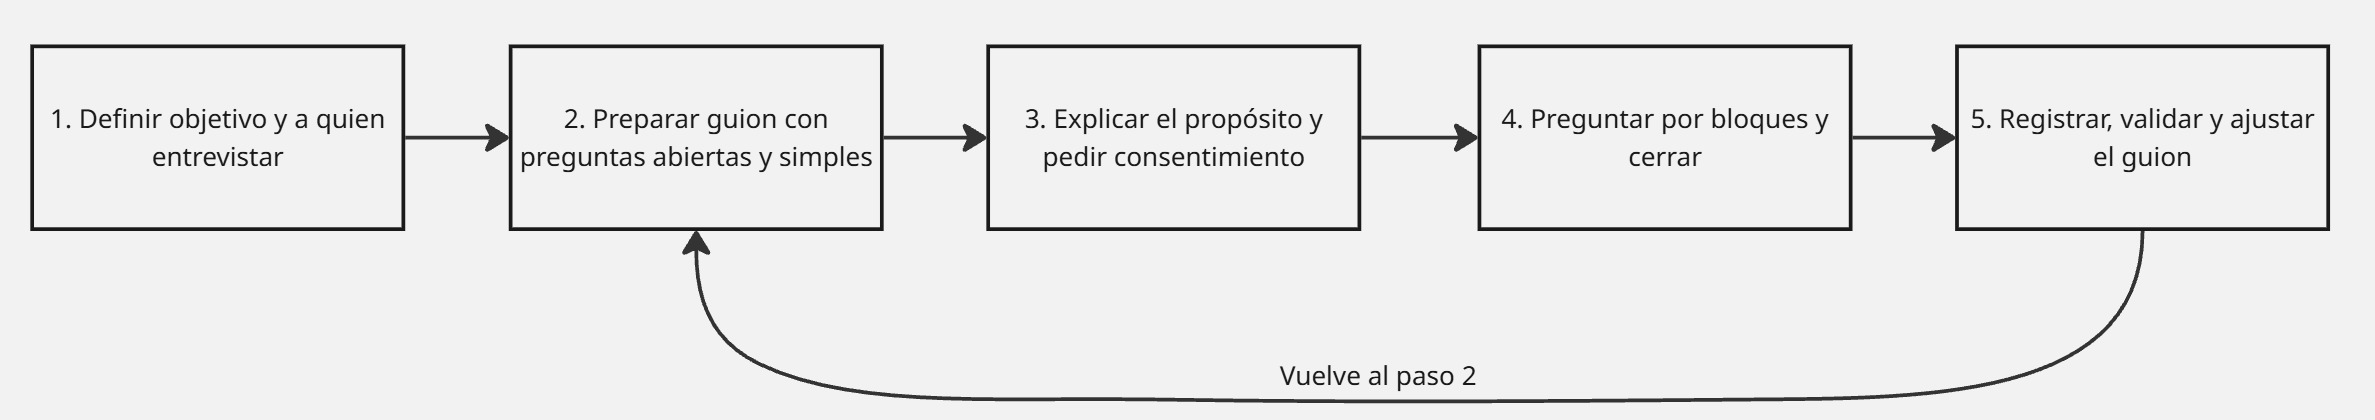
\includegraphics[width=\textwidth]{figuras/flujo-entrevista.jpg}

  \raggedright
  \vspace{10pt}
  \textbf{Cuándo:} pocos stakeholders clave y detalle individual \cite[Sec.~19.2, pp.~245--255]{pohl2025}
\end{frame}

\begin{frame}{Entrevista: ventajas, limitaciones y ejemplo propio}
  \small
  \begin{columns}[T]
    \begin{column}{0.48\textwidth}
      \textbf{Ventajas}
      \begin{itemize}
        \item Más fácil de agendar que un taller grande \cite[Cap.~7, pp.~121--122]{wiegers2013}
        \item Permite repreguntar en el momento.
      \end{itemize}
      \textbf{Limitaciones}
      \begin{itemize}
        \item Solo sale lo que el entrevistado sabe decir.
        \item Preguntas inductivas o dobles sesgan.
      \end{itemize}
    \end{column}
    \begin{column}{0.48\textwidth}
      \textbf{Ejemplo propio (GA-TL-02, P3)}
      \begin{itemize}
        \item \textbf{Original:} «¿Qué problemas o atrasos les da trabajar con las hojas impresas de inscripción?»
        \item \textbf{Defecto:} inductiva y doble.
        \item \textbf{Corregida:} «¿Cómo es su experiencia trabajando con las hojas impresas de inscripción?»
      \end{itemize}
    \end{column}
  \end{columns}
\end{frame}


% ============ BLOQUE B: herramientas automatizadas ============
% BLOQUE B -- Comparación de herramientas (responsable: Lavayen).
% Datos de la tabla tomados de las páginas oficiales citadas.
% Evidencia propia: Issues #1 (RF-01) y #2 (TC-01) del repositorio del equipo.
\begin{frame}{Herramienta pesada frente a ligera: Helix ALM y GitHub Issues}
  \begin{columns}[T]
    \begin{column}{0.55\textwidth}
      \scriptsize
      \renewcommand{\arraystretch}{1.15}
      \begin{tabular}{@{}p{1.5cm}p{2.6cm}p{2.6cm}@{}}
        \toprule
         & \textbf{Helix ALM}\newline{\tiny(hoy Perforce ALM)} & \textbf{GitHub Issues} \\
        \midrule
        Enfoque & Módulos de requisitos, pruebas e incidencias \cite{perforcealm2026} & Seguimiento de tareas, ideas y errores en el repositorio \cite{githubissues2026} \\
        Trazabilidad & Matriz de trazabilidad automática \cite{perforcealm2026} & Referencias por mención (\#n), sub-issues y dependencias \cite{githubissues2026} \\
        Costo & Precio no publicado; prueba de 30 días \cite{perforcealm2026} & Sin costo en nuestro repositorio público (uso propio) \\
        No conviene si\ldots & El equipo tiene presupuesto limitado y plazos de entrega reducidos, ya que es costoso y complejo de usar & El proyecto exige documentación extensa y trazabilidad formal para auditorías \\
        \bottomrule
      \end{tabular}
    \end{column}
    \begin{column}{0.43\textwidth}
      \centering
      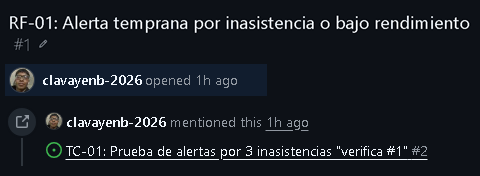
\includegraphics[width=\linewidth,height=0.62\textheight,keepaspectratio]{figuras/issues-rf01-recorte.png}

      \vspace{2pt}
      {\scriptsize Ejemplo propio: RF-01 (\#1) enlazado con su prueba TC-01 (\#2).}
    \end{column}
  \end{columns}

  \vspace{4pt}
  \footnotesize\textbf{Conclusión:} para nuestro proyecto de fin de curso conviene GitHub Issues, ya que es el más óptimo para nosotros como estudiantes de la carrera.
\end{frame}


% ============ BLOQUES C y D: recomendación y demostración ============
\documentclass[aspectratio=169]{beamer}
\usepackage[utf8]{inputenc}
\usepackage[T1]{fontenc}
\usepackage[spanish]{babel}
\usepackage{tikz}
\usepackage{booktabs}
\usetikzlibrary{arrows.meta, positioning}

\usetheme{Madrid}
\usecolortheme{seahorse}

\title{Helix ALM}
\author{Jordy Fabi\'an Rivas Bodero}
\institute{UTEQ --- Ingenier\'ia de Requerimientos (ISR-401)}
\date{Noviembre 2026}

\begin{document}

\begin{frame}
  \titlepage
\end{frame}

\begin{frame}{Helix ALM: Evaluaci\'on de Adopci\'on}
  \begin{block}{Uso en Equipos \'Agiles}
    \begin{itemize}
      \item No conviene imponer Helix ALM como eje diario cuando se busca iteraci\'on r\'apida y baja carga administrativa \cite{pohl2015requirements}.
      \item Implica costo de licenciamiento, curva de aprendizaje y mantenimiento de flujos y enlaces \cite{pohl2015requirements}.
      \item En entornos livianos resulta preferible un flujo \'agil directo con \textbf{Git + Markdown + Issues}.
    \end{itemize}
  \end{block}
  \vspace{0.2cm}
  \begin{alertblock}{Entornos Cr\'iticos o Regulados}
    \begin{itemize}
      \item Resulta adecuado cuando se exigen auditor\'ias formales, cumplimiento normativo o trazabilidad estricta \cite{pohl2015requirements}.
    \end{itemize}
  \end{alertblock}
\end{frame}

\begin{frame}{Helix ALM: Veredicto T\'ecnico}
  \begin{columns}[T]
    \begin{column}{0.48\textwidth}
      \begin{block}{Cu\'ando Evitarlo}
        \begin{itemize}
          \item Equipos peque\~nos o prototipos con alta velocidad de cambio.
          \item Cuando la configuraci\'on de \'items supera el beneficio operativo.
          \item Presupuestos ajustados sin necesidad de certificaci\'on formal.
        \end{itemize}
      \end{block}
    \end{column}
    \begin{column}{0.48\textwidth}
      \begin{block}{Cu\'ando Aplicarlo}
        \begin{itemize}
          \item Gesti\'on centralizada de requisitos, casos de prueba e incidencias \cite{pohl2015requirements}.
          \item Trazabilidad bidireccional auditable entre artefactos \cite{pohl2015requirements}.
          \item An\'alisis de impacto ante modificaciones \cite{pohl2015requirements}.
        \end{itemize}
      \end{block}
    \end{column}
  \end{columns}
\end{frame}

\begin{frame}{Helix ALM: Trazabilidad de \'Items}
  \begin{center}
    \begin{tikzpicture}[
      node distance=1.4cm,
      box/.style={rectangle, draw=blue!60!black, fill=blue!8, thick, rounded corners, minimum width=3.4cm, minimum height=1.5cm, align=center, font=\small},
      arrow/.style={-{Stealth[length=3mm]}, thick, blue!70!black}
    ]
      \node[box] (req) {\textbf{Requisito (REQ-01)}\\Especificaci\'on de regla\\o condici\'on funcional\\del sistema};
      \node[box, right=of req] (tc) {\textbf{Caso de Prueba (TC-01)}\\Verificaci\'on del\\comportamiento y\\criterios de salida};
      \node[box, right=of tc] (inc) {\textbf{Incidencia (INC-01)}\\Registro de defecto o\\desviaci\'on detectada\\en ejecuci\'on};

      \draw[arrow] (req) -- node[above, font=\scriptsize] {Verifica} (tc);
      \draw[arrow] (tc) -- node[above, font=\scriptsize] {Genera} (inc);
      \draw[arrow, dashed, red!70!black] (inc.south) to[bend left=22] node[below, font=\scriptsize] {Impacta / Revisi\'on} (req.south);
    \end{tikzpicture}
  \end{center}

  \vspace{0.2cm}
  \begin{itemize}
    \item Enlaza requisitos, casos de prueba e incidencias dentro de un mismo repositorio de gesti\'on \cite{pohl2015requirements}.
  \end{itemize}
\end{frame}

\begin{frame}{Helix ALM: Matriz de Impacto}
  \begin{table}
    \centering
    \small
    \begin{tabular}{llll}
      \toprule
      \textbf{Artefacto} & \textbf{ID} & \textbf{Estado Anterior} & \textbf{Acci\'on por Alerta de Impacto} \\
      \midrule
      Requisito & REQ-01 & Aprobado (v1.0) & Actualizado a v1.1 (nuevo criterio) \\
      Caso de Prueba & TC-01 & Aprobado & Marcado como \textit{Sospechoso} (re-ejecutar) \\
      Incidencia & INC-01 & En revisi\'on & Reevaluar causa y alcance del cambio \\
      \bottomrule
    \end{tabular}
  \end{table}

  \vspace{0.2cm}
  \begin{block}{Propagaci\'on de Cambios}
    Helix ALM marca como \textit{sospechosos} los \'items vinculados cuando se modifica un elemento relacionado \cite{pohl2015requirements}.
  \end{block}
\end{frame}

\begin{frame}{Helix ALM: Conclusiones}
  \begin{block}{S\'intesis}
    \begin{itemize}
      \item Helix ALM aporta trazabilidad formal y control de impacto sobre requisitos, pruebas e incidencias \cite{pohl2015requirements}.
      \item Su adopci\'on debe evaluarse frente al costo operativo y al nivel de formalidad exigido \cite{pohl2015requirements}.
    \end{itemize}
  \end{block}
\end{frame}

\begin{frame}[allowframebreaks]{Referencias}
  \footnotesize
  \bibliographystyle{IEEEtran}
  \bibliography{referencias/referencias}
\end{frame}

\end{document}

% ============ DECLARACIÓN DE USO DE IA ============
\begin{frame}{Declaración de uso de herramientas de IA}
  % Obligatoria. Si no se usó ninguna, escribirlo así.
  \textcolor{red}{[Pendiente por llenar]}
\end{frame}

% ============ REFERENCIAS (IEEE, última diapositiva) ============
\begin{frame}[allowframebreaks]{Referencias}
  \footnotesize
  \bibliographystyle{IEEEtran}
  \bibliography{referencias/referencias}
\end{frame}

\end{document}
